
% Set document class and font size
\documentclass[letterpaper, 11pt]{article}
\usepackage[utf8]{inputenc}

% Package imports
\usepackage{setspace, longtable, graphicx, hyphenat, hyperref, fancyhdr, ifthen, everypage, enumitem, amsmath, setspace}
\usepackage{array}
\usepackage{tabularx}

\makeatletter
\newcommand*\bigcdot{\mathpalette\bigcdot@{1.0}}
\newcommand*\bigcdot@[2]{\mathbin{\vcenter{\hbox{\scalebox{#2}{$\m@th#1\bullet$}}}}}
\makeatother

\usepackage[]{biblatex}
\addbibresource{sample.bib}

% --- Page layout settings ---

% Set page margins
\usepackage[left=1.5cm, right=1.5cm, bottom=1.0cm, top=1.0cm]{geometry}

% --- Page formatting ---

% Set link colors
\usepackage[dvipsnames]{xcolor}
\urlstyle{sf}
\hypersetup{colorlinks=true, linkcolor=Blue, urlcolor=Blue}

% Set font to Libertine, including math support
\usepackage{libertine}
\usepackage[libertine]{newtxmath}

% Remove page numbering
\pagenumbering{gobble}

% --- Document starts here ---

\begin{document}


% set no indent
\setlength\parindent{0pt}\textbf{}

\hfill%
\begin{minipage}{0.79\textwidth}\flushleft
\huge{\bf{Eliott Johnson}}\\
\normalsize
12 Sep, 1993 $\bigcdot$ 8A ch. de Challendin, CH-1224 Chêne-bougeries $\bigcdot$ Suisse \\
+41 (0) 79 396 28 27 $\bigcdot$  \href{mailto:eliott.johnson@gmail.com}{eliott.johnson@gmail.com} $\bigcdot$  \href{https://www.linkedin.com/in/eliottjohnson/}{Linkedin: eliottjohnson}\\
\href{https://www.eliottjohnson.ch}{Website: www.eliottjohnson.ch}
\end{minipage}
\begin{minipage}{0.19\textwidth}% adapt widths of minipages to your needs
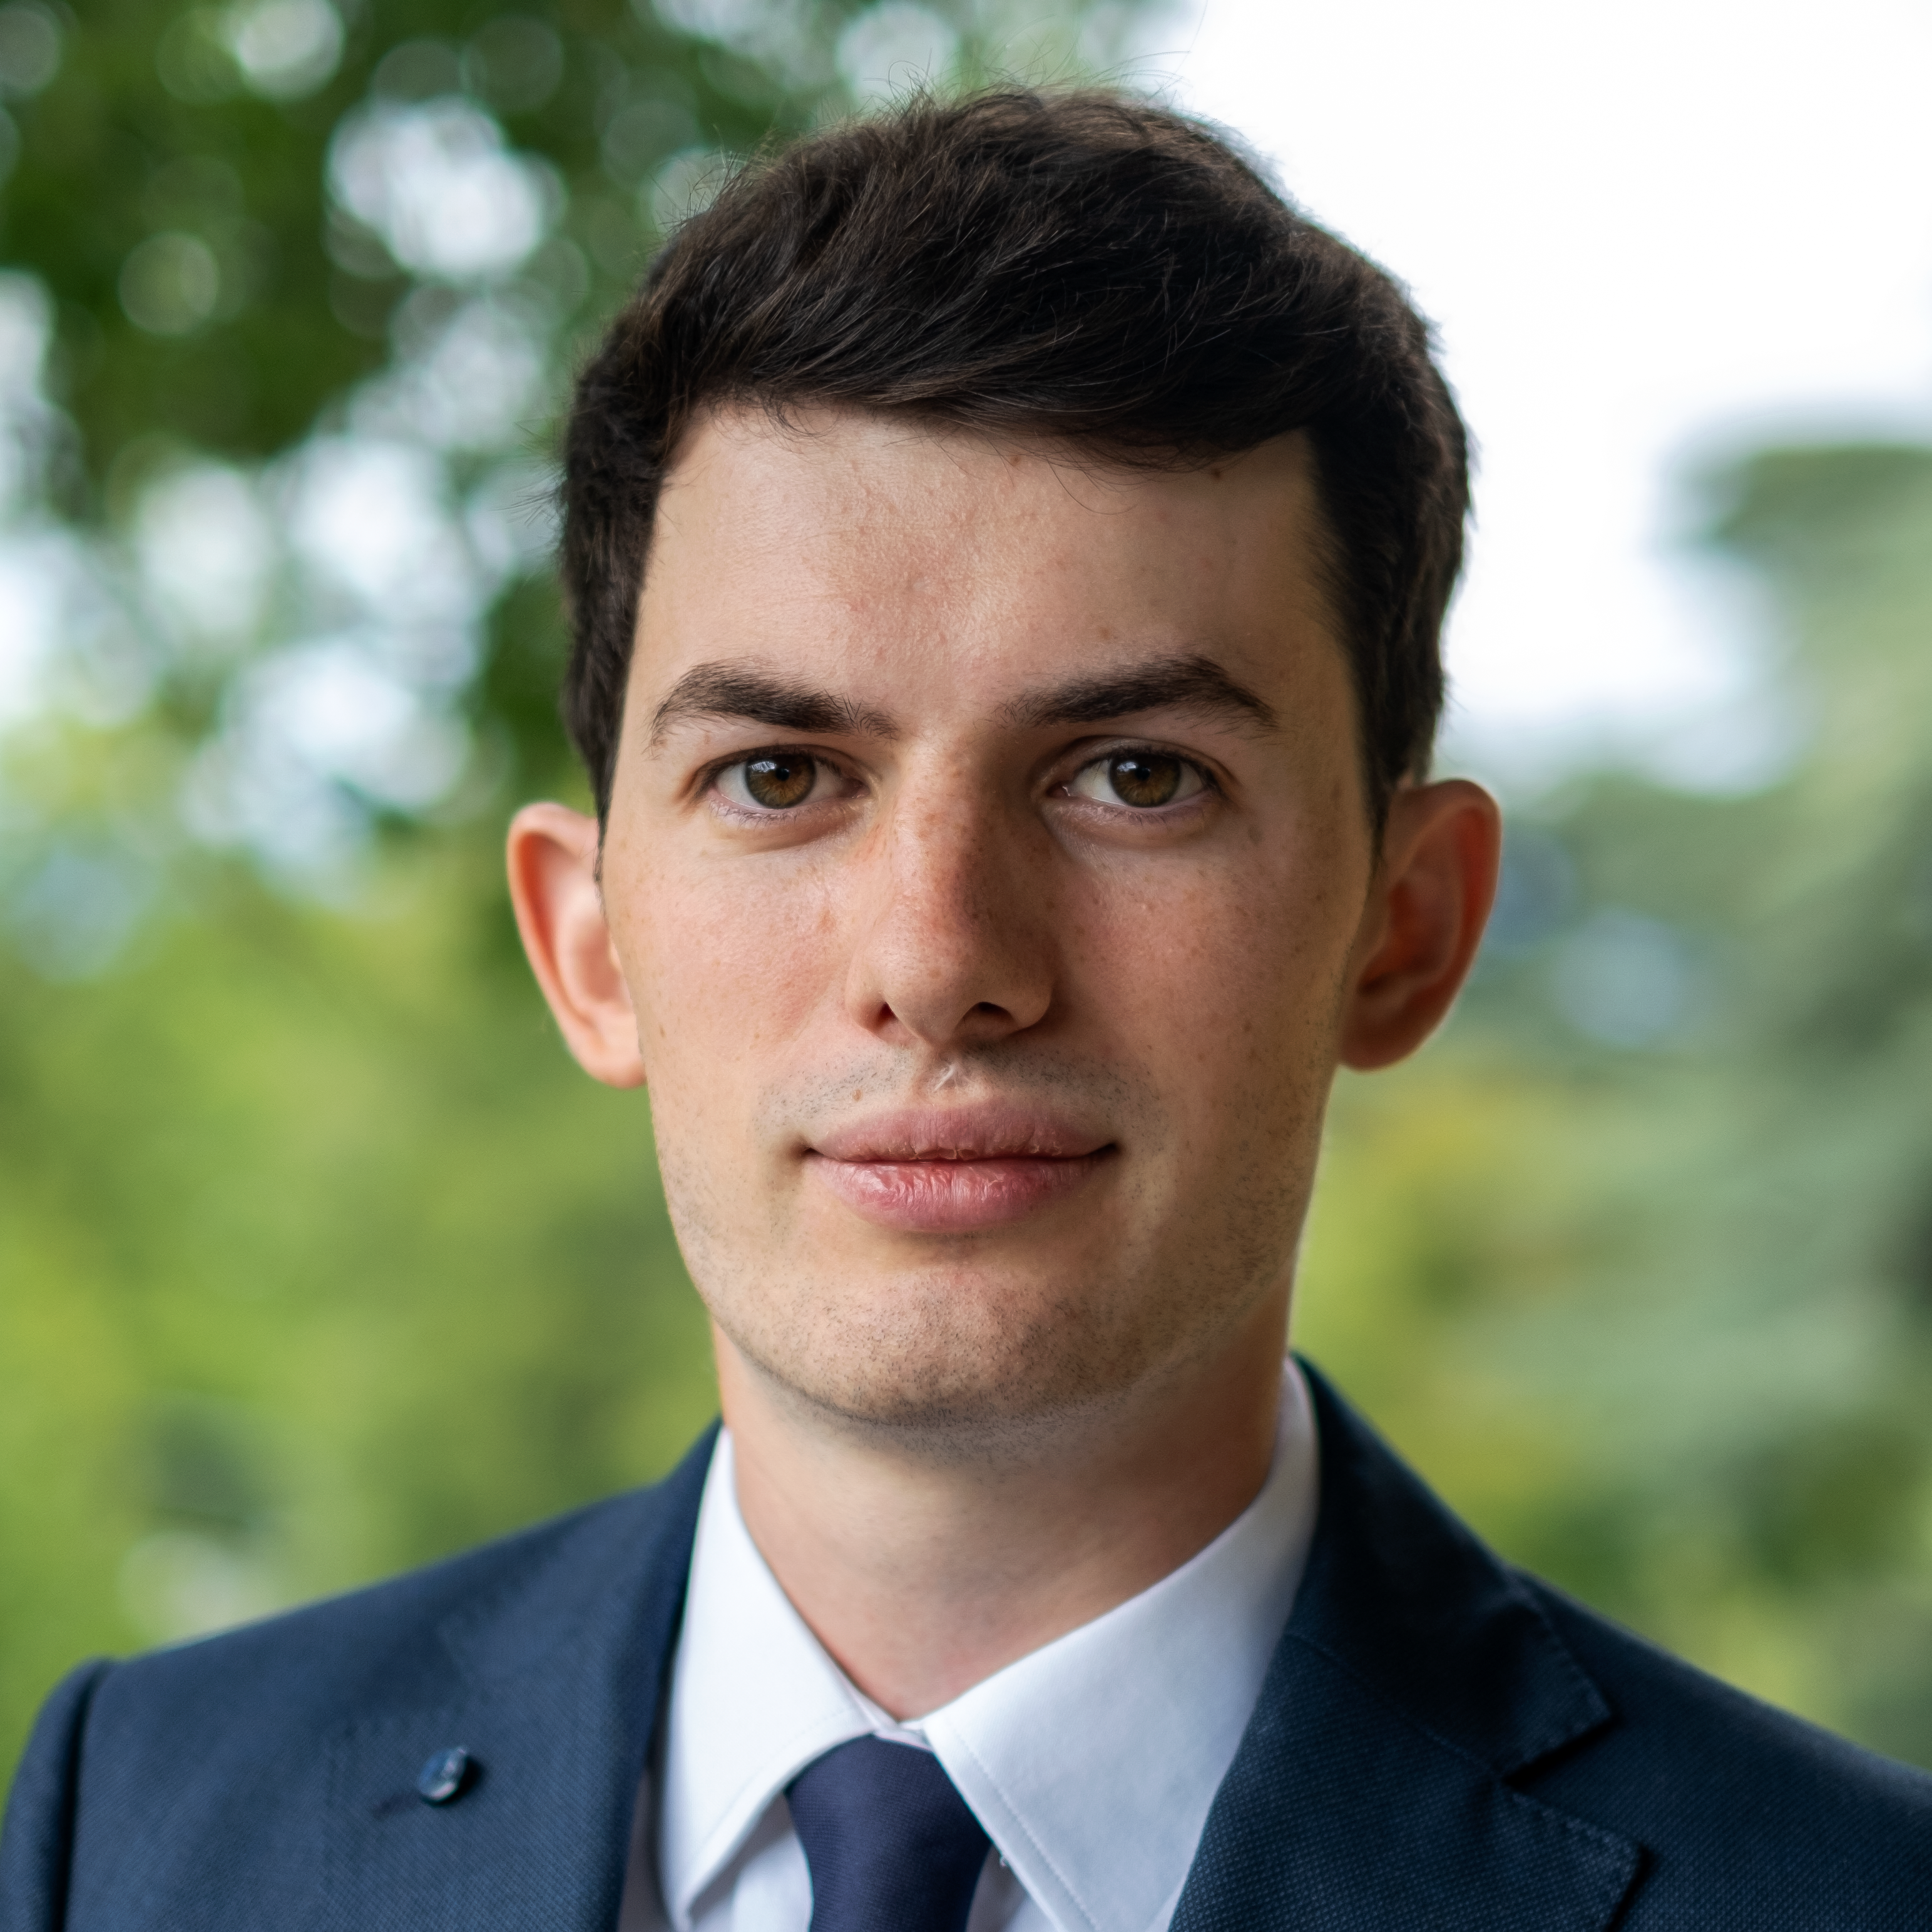
\includegraphics[width=\linewidth]{LinkedInProfilPic.png}
\end{minipage}%
\vspace{0.25cm}

\noindent\rule{\textwidth}{1pt}

% --- Section: Education ---
\begin{center}
\large\bf{FORMATION}
\end{center}

\begin{tabularx}{1.0\textwidth} { 
   >{\raggedright\arraybackslash\hsize=1.5\hsize\linewidth=\hsize}X 
   >{\raggedleft\arraybackslash\hsize=.5\hsize\linewidth=\hsize}X }
\normalsize
\bf{Université de Genève} & Genève, CH \\
\normalfont Maîtrise universitaire\ en physique des particules & Sep 2018 -- Juin 2020  \\  
Électrodynamique quantique, Chromodynamique quantique, Théorie quantique des champs, Relativité générale, Physique des rayonnements cosmiques, Détecteurs et accélérateurs &
\end{tabularx}
\vspace{0.25cm}

\begin{tabularx}{1.0\textwidth} { 
   >{\raggedright\arraybackslash\hsize=1.5\hsize\linewidth=\hsize}X 
   >{\raggedleft\arraybackslash\hsize=.5\hsize\linewidth=\hsize}X }
\normalsize
\bf{Université de Goettingen} & Goettingen, GER \\
\normalfont Hadron collider physics school (HASCO) & Juil 2018 \\
International Student Exchange Program
\end{tabularx}
\vspace{0.25cm}

\begin{tabularx}{1.0\textwidth} { 
   >{\raggedright\arraybackslash\hsize=1.5\hsize\linewidth=\hsize}X 
   >{\raggedleft\arraybackslash\hsize=.5\hsize\linewidth=\hsize}X }
\normalsize
\bf{Université de Genève} & Genève, CH \\
\normalfont Baccalauréat universitaire\ en Physique & Sep 2015 -- Juin 2018  \\  
Mécanique newtonienne, Électrodynamique, Algèbre linéaire, Analyse complexe \& de Fourier, Astrophysiques, Mécanique statistique et Physique du solide &
\end{tabularx}
\vspace{0.25cm}

\begin{tabularx}{1.0\textwidth} { 
   >{\raggedright\arraybackslash\hsize=1.5\hsize\linewidth=\hsize}X 
   >{\raggedleft\arraybackslash\hsize=.5\hsize\linewidth=\hsize}X }
\normalsize
\bf{École Polytechnique Fédérale de Lausanne (EPFL)} & Lausanne, CH \\
\normalfont Génie mécanique & Sep 2014 -- Juin 2015\\
Analyse, Algèbre linéaire, Mécanique newtonienne, Thermodynamique, 
Construction mécanique, Enjeux mondiaux, Communication, Mécanique des structures, Matériaux, Électricité
\end{tabularx}
\vspace{0.25cm}

\begin{tabularx}{1.0\textwidth} { 
   >{\raggedright\arraybackslash\hsize=1.5\hsize\linewidth=\hsize}X 
   >{\raggedleft\arraybackslash\hsize=.5\hsize\linewidth=\hsize}X }
\normalsize
\bf{École Polytechnique Fédérale de Zürich (ETH)} & Zürich, CH \\
\normalfont Génie mécanique & Sep 2013 -- Juin 2014 \\
Analyse, Algèbre linéaire, Mécanique newtonienne, Matériaux et fabrication, Dessin technique \& CAD, Chimie, Éléments de machine, Informatique, Processus d'innovation \& projet
\end{tabularx}
\vspace{0.25cm}

% --- Section: Work Experience ---
\begin{center}
\noindent\rule{0.75\textwidth}{1pt}
\end{center}

\begin{center}
\large\bf{EXPÉRIENCE PROFESSIONNELLE}
\end{center}

\begin{tabularx}{1.0\textwidth} { 
   >{\raggedright\arraybackslash\hsize=1.5\hsize\linewidth=\hsize}X 
   >{\raggedleft\arraybackslash\hsize=.5\hsize\linewidth=\hsize}X }
\normalsize
\bf{Agent d'escale - Swissport} & Genève, CH\\
\normalfont \begin{itemize}[leftmargin=*,noitemsep,topsep=0pt]
\item Responsable de tous mouvements de passagers entre le terminal et l'avion ainsi que du traitement des documents de voyage et de l'attribution des cartes d'embarquement
\item Habilitation de sécurité et permis de conduire pour tarmac sur aéroport international
\item Horaires irréguliers (soir, nuits, WE, jours fériés)
\end{itemize} & Nov 2018 -- Aujourd'hui
\end{tabularx}

\begin{tabularx}{1.0\textwidth} { 
   >{\raggedright\arraybackslash\hsize=1.5\hsize\linewidth=\hsize}X 
   >{\raggedleft\arraybackslash\hsize=.5\hsize\linewidth=\hsize}X }
\normalsize
\bf{Organisation européenne pour la recherche nucléaire (CERN)} & Genève, CH\\
\normalfont \begin{itemize}[leftmargin=*,noitemsep,topsep=0pt]
\item 
Participation à la création de FASER, une nouvelle expérience qui se focalise sur les particules massives faiblement interactives
\item Assurance qualité et programmation du système de déclenchement du signal
\item Intégration de mon design dans le flux de travail d'une équipe de plus de 30 scientifiques internationaux
\end{itemize} & Sep 2019 -- Juil 2020
\end{tabularx}

\begin{tabularx}{1.0\textwidth} { 
   >{\raggedright\arraybackslash\hsize=1.5\hsize\linewidth=\hsize}X 
   >{\raggedleft\arraybackslash\hsize=.5\hsize\linewidth=\hsize}X }
\normalsize
\bf{
Assistant de laboratoire de physique - Université de Genève \& ECG Jean-Piaget} & Genève, CH\\
\normalfont \begin{itemize}[leftmargin=*,noitemsep,topsep=0pt]
\item Encadrement d'étudiants du secondaire et de l'université pour acquérir et analyser des données à l'aide d'expériences pratiques
\end{itemize} & Sep 2018 -- Août 2020
\end{tabularx}

\begin{tabularx}{1.0\textwidth} { 
   >{\raggedright\arraybackslash\hsize=1.5\hsize\linewidth=\hsize}X 
   >{\raggedleft\arraybackslash\hsize=.5\hsize\linewidth=\hsize}X }
\normalsize
\bf{
Stage en génie mécanique - Rolex} & Genève, CH\\
\normalfont \begin{itemize}[leftmargin=*,noitemsep,topsep=0pt]
\item Participation aux différentes étapes de la création de montres haut de gamme, de la fusion de l'or à la cuisson de la céramique
\end{itemize} & Jan 2014 --  Féb 2014
\end{tabularx}

\begin{tabularx}{1.0\textwidth} { 
   >{\raggedright\arraybackslash\hsize=1.5\hsize\linewidth=\hsize}X 
   >{\raggedleft\arraybackslash\hsize=.5\hsize\linewidth=\hsize}X }
\normalsize
\bf{Armée Suisse - 
Escadron d'aviation 14} & Payerne \& Sion, CH\\
\normalfont \begin{itemize}[leftmargin=*,noitemsep,topsep=0pt]
\item Soldat d'aviation sur les F-5 Tiger et les F-18 Hornet
\item Préparation du système de navigation inertielle embarqué des avions, ravitaillement et signalisation manuelle de la procédure de démarrage
\end{itemize} & Juil 2012 -- Déc 2012
\end{tabularx}

% --- Section: Additional Experience ---
\begin{center}
\noindent\rule{0.75\textwidth}{1pt}
\end{center}

\begin{center}
\large\bf{EXPÉRIENCE SUPPLÉMENTAIRE}
\end{center}

\begin{tabularx}{1.0\textwidth} { 
   >{\raggedright\arraybackslash\hsize=1.5\hsize\linewidth=\hsize}X 
   >{\raggedleft\arraybackslash\hsize=.5\hsize\linewidth=\hsize}X }
\normalsize
\bf{Expert en radioprotection - CHUV} & Lausanne, CH\\
\normalfont \begin{itemize}[leftmargin=*,noitemsep,topsep=0pt]
\item Qualifié en tant qu'expert en radioprotection dans l'utilisation de matières radioactives non scellées dans une zone de travail B/C
\end{itemize} & Féb -- Juil 2019
\end{tabularx}

\begin{tabularx}{1.0\textwidth} { 
   >{\raggedright\arraybackslash\hsize=1.5\hsize\linewidth=\hsize}X 
   >{\raggedleft\arraybackslash\hsize=.5\hsize\linewidth=\hsize}X }
\normalsize
\bf{
Passionné d'aviation} & Grenchen, CH\\
\normalfont \begin{itemize}[leftmargin=*,noitemsep,topsep=0pt]
\item Licence de pilote privé (PPL) et voltige
\item Recommandé par SPHAIR pour devenir pilote commercial et/ou militaire
\item Participé à trois reprises au championnat national suisse de voltige
\end{itemize} & 2014
\end{tabularx}


% --- Section: Skills ---
\begin{center}
\noindent\rule{0.75\textwidth}{1pt}
\end{center}

\begin{center}
\large\bf{COMPÉTENCES}
\end{center}

\begin{tabularx}{1.0\textwidth} { 
   >{\raggedright\arraybackslash\hsize=1.5\hsize\linewidth=\hsize}X 
   >{\raggedleft\arraybackslash\hsize=.5\hsize\linewidth=\hsize}X }
\normalsize
\bf{Langues} & \\
\normalfont
Français - Langue maternelle & \\
Anglais - Bilingue & \\
Allemand - Bonnes connaissances 
\end{tabularx}
\vspace{0.25cm}

\begin{tabularx}{1.0\textwidth} { 
   >{\raggedright\arraybackslash\hsize=1.5\hsize\linewidth=\hsize}X 
   >{\raggedleft\arraybackslash\hsize=.5\hsize\linewidth=\hsize}X }
\normalsize
\bf{Compétences informatiques} & \\
\normalfont \begin{itemize}[leftmargin=*,noitemsep,topsep=0pt]
\item \textbf{Suite Microsoft Office:}  Excel, Word, PowerPoint, Outlook
\item \textbf{Programmation:} C++, Python, Github (version control), HTML, CSS
\item \textbf{Analyse des données:} SQL, Mathematica, Matlab, Root, Igor
\item \textbf{Autre:} Linux, LateX, CAD, Arduino, 3D printing, Adobe Premiere, Construction d'ordinateur
\end{itemize} & 
\end{tabularx}

% --- Section: Publication ---
\begin{center}
\noindent\rule{0.75\textwidth}{1pt}
\end{center}

\begin{center}
\large\bf{PUBLICATION}
\end{center}

\nocite{*}

\printbibliography[title=\normalsize Thèse de maîtrise universitaire]

% --- End of CV! ---


\end{document}
